\documentclass[../../main.tex]{subfiles}
\begin{document}

\begin{flushright}
\footnotesize\textit{【自動文字起こし・要確認】}
\end{flushright}

\noindent
\textbf{[解]} $S_1 - \int_1^a \log x \, dx = a(\log a - 1) + 1 \quad \dots \text{① である.}$

\bigskip

(1) $\square ABCD$ の面積を $S'$ とすると,
\[
S' = \triangle ABD D' + \triangle D' B C = \dfrac{1}{2}(\log a + \log b)(a - b) + \dfrac{1}{2} \log b \cdot (b - 1)
\]
図より明らかに $S' < S_1$ だから, $S'$ の最大値こそ $S_2$ である.

\begin{center}
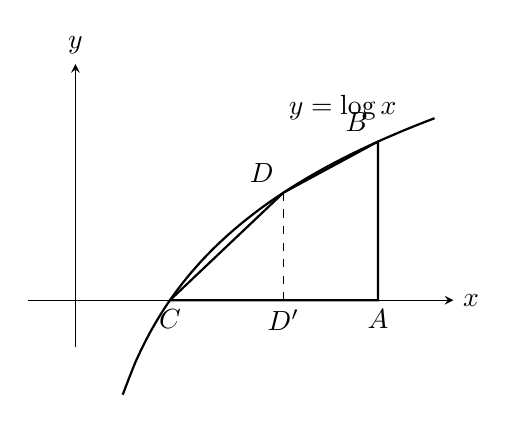
\begin{tikzpicture}[scale=1.2, >=stealth]
\draw[->] (-0.5,0) -- (4,0) node[right] {$x$};
\draw[->] (0,-0.5) -- (0,2.5) node[above] {$y$};
\draw[domain=0.5:3.8, smooth, variable=\x, thick] plot ({\x}, {log2(\x)});
\node[above left] at (3.5, {log2(3.5)}) {$y = \log x$};
\coordinate (C) at (1,0);
\coordinate (Dp) at (2.2,0);
\coordinate (A) at (3.2,0);
\coordinate (D) at (2.2,{log2(2.2)});
\coordinate (B) at (3.2,{log2(3.2)});

\draw[dashed] (D) -- (Dp);
\draw[dashed] (B) -- (A);
\draw[thick] (C) -- (D) -- (B) -- (A) -- cycle;

\node[below] at (C) {$C$};
\node[below] at (Dp) {$D'$};
\node[below] at (A) {$A$};
\node[above left] at (D) {$D$};
\node[above left] at (B) {$B$};
\end{tikzpicture}
\end{center}

\[
\dfrac{d}{db} S' = \dfrac{1}{2b}(a - 1) - \dfrac{1}{2} \log a
\]
より, 極大を与える $\left(\because \dfrac{a-1}{\log a} < a\right)$

\begin{center}
\begin{tabular}{c|ccccc}
$b$ & $(1)$ & $\dots$ & $\dfrac{a-1}{\log a}$ & $\dots$ & $a$ \\ \hline
$S'$ & & $+$ & $0$ & $-$ & \\ \hline
$S$ & & $\nearrow$ & 極大 & $\searrow$ & 
\end{tabular}
\end{center}

従って,
\[
S_2 = S'\Big|_{b = \dfrac{a-1}{\log a}} = \dfrac{1}{2}(a \log a - a + 1) + \dfrac{1}{2} \dfrac{a-1}{\log a} \log\left(\dfrac{a-1}{\log a}\right)
\]

\bigskip

(2)
\begin{align}
\dfrac{S_2}{S_1} &= \dfrac{\dfrac{1}{2}(a \log a - a + 1) + \dfrac{1}{2}(a-1)\{\log(a-1) - \log\log a\}}{a \log a - a + 1} \\
&= \dfrac{1}{2} + \dfrac{1}{2} \underbrace{\dfrac{(a-1)\{\log(a-1) - \log\log a\}}{a \log a - a + 1}}_{T}
\end{align}

\[
T = \dfrac{\left(1 - \dfrac{1}{a}\right) \left\{ 1 + \dfrac{\log(1 - \dfrac{1}{a})}{\log a} - \dfrac{\log\log a}{\log a} \right\}}{1 - \dfrac{1}{\log a} + \dfrac{1}{a \log a}} \longrightarrow 1 \quad (a \to \infty)
\]
\[
\left[ \log a = A \to \infty \text{ より } \dfrac{\log(\log a)}{\log a} = \dfrac{\log A}{A} \to 0 \right]
\]
より,
\[
\dfrac{S_2}{S_1} \longrightarrow 1 \quad (a \to \infty) \text{ である.}
\]

\newpage

\end{document}
